\recipe{Crepes}
\label{recipe:crepes}
\worktime{10 minutes}
\totaltime{30 minutes}
\makes{Makes enough for one hungry person}
\source{https://www.bbcgoodfood.com/recipes/easy-pancakes-two-ways}

\begin{ingredients}
    \item \SI{100}{\gram} plain flour
    \item \SI{300}{\milli \litre} milk
    \item 2 Eggs
    \item Butter for cooking
    \ingroup{Topping Suggestions}
    \item Lemon \& Sugar
    \item Nutella
    \item syrup \& Banana
    
\end{ingredients}

\begin{method}
Slowly add wet ingredients to dry ingredients while mixing.

Fry.
\end{method}


\begin{figure}[h]
  	\centering
  	
  	\begin{tikzpicture}
  		% Save the image in a box to get its dimensions
  		\sbox0{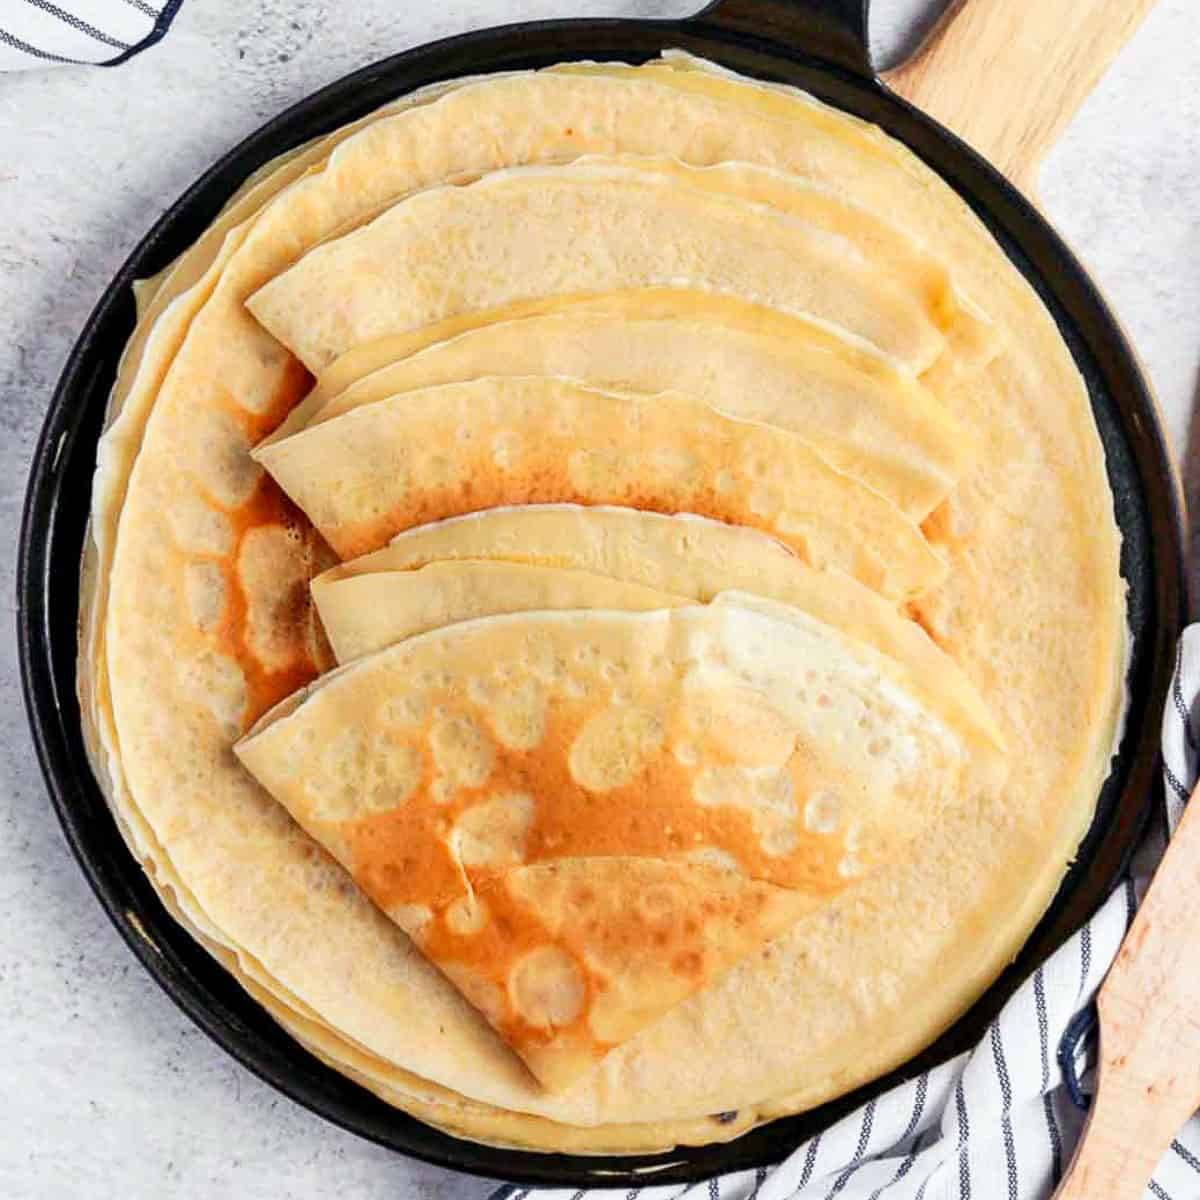
\includegraphics[width=0.9\linewidth]{images/French-Crepes-Feature1.jpg}}%
  
  		% Draw a clipping rectangle with rounded corners
  		\path[clip, rounded corners=0.5cm] (0,0) rectangle (\wd0,\ht0);
  
  		% Place the image inside the clipped area
  		\node[inner sep=0pt, outer sep=0pt, anchor=south west] at (0,0) {\usebox0};
	\end{tikzpicture}

  \caption*{}
\end{figure}